\documentclass{article}
\usepackage{tikz}
\usepackage{geometry}
\usetikzlibrary{positioning}

% Set page margins to show the entire diagram
\geometry{margin=0pt}

\begin{document}
\vspace*{1cm} % Adjust the value as needed to lower the diagram
\begin{center} % Center the diagram
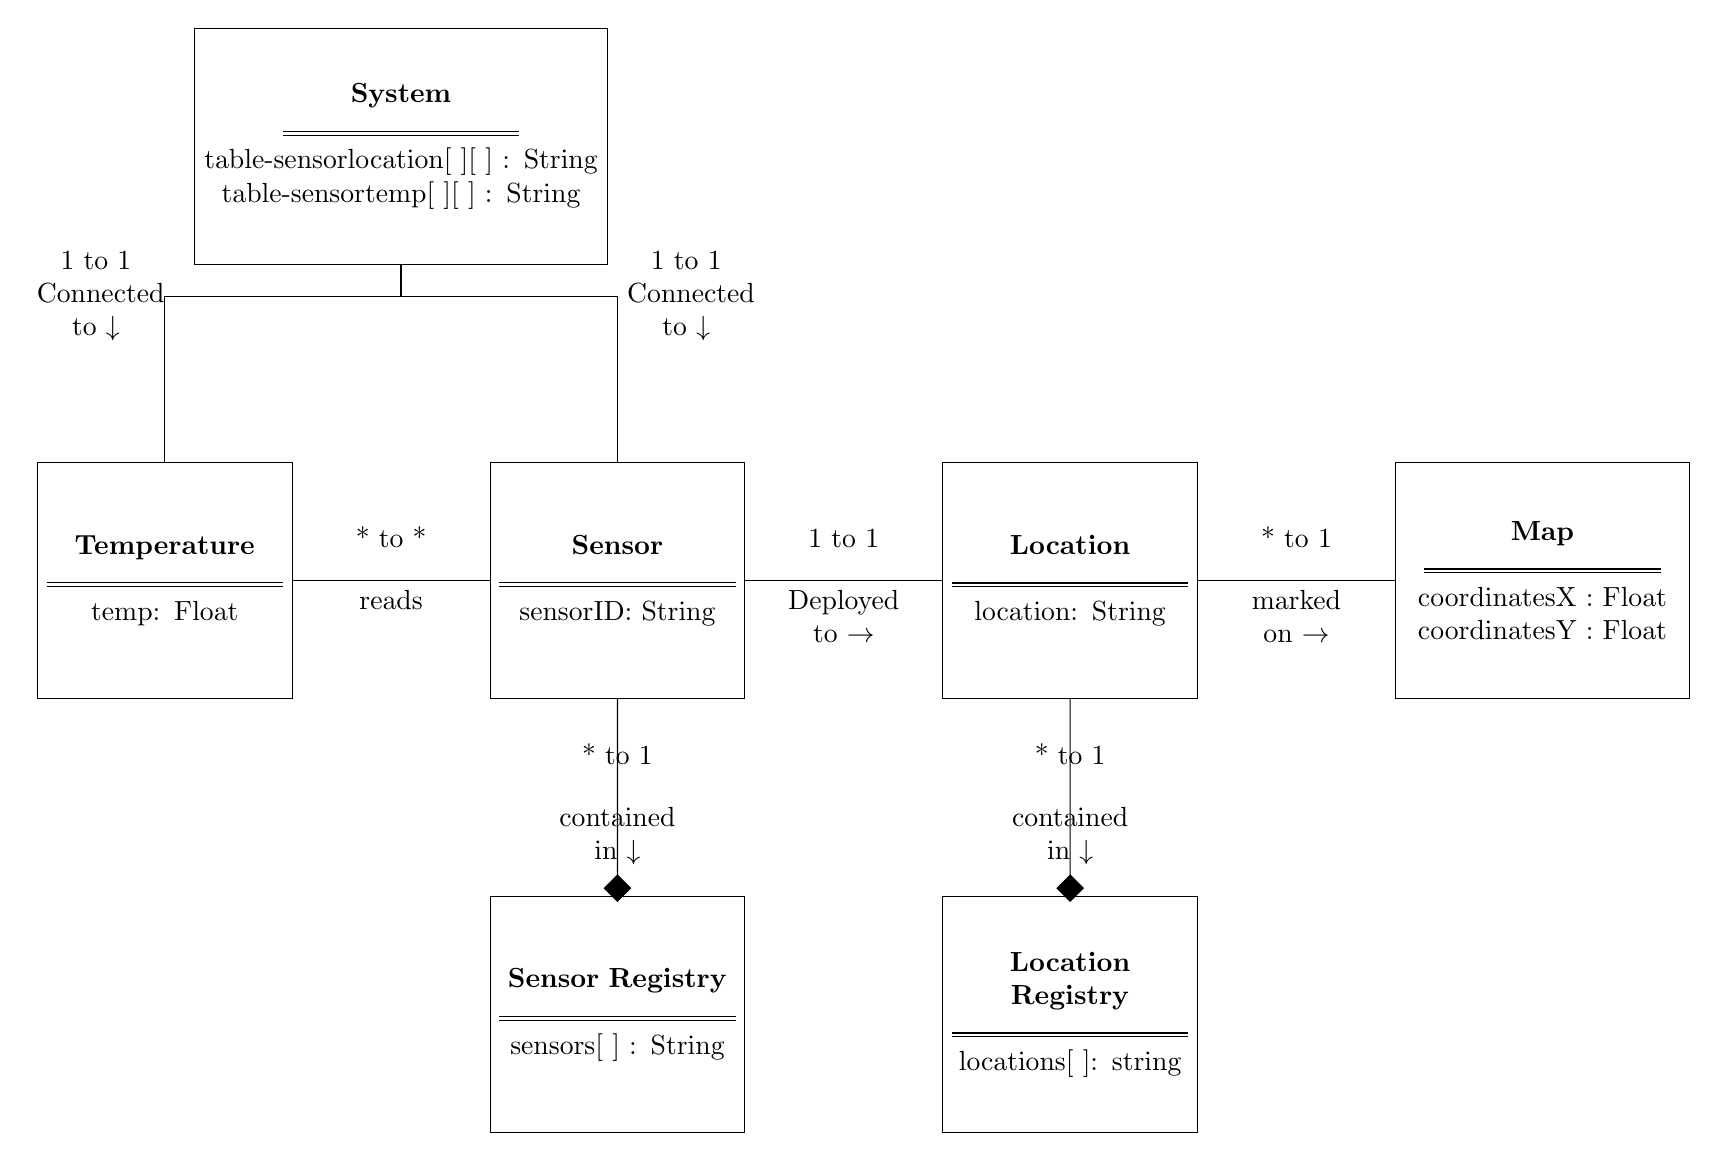
\begin{tikzpicture}[
    node distance = 2.5cm,
    scale=0.8, % Adjust the scale as needed to fit the diagram on the page
]

% Define a command for drawing horizontal lines in nodes
\newcommand{\horizontalline}{\hspace*{0pt}\vbox{\hrule width 3cm\kern1pt\hrule width 3cm}}

% Nodes with horizontal lines and text in the upper half
\node[draw, text width=3cm, align=center, minimum height=3cm] (temperature) {
    \textbf{Temperature}\\
    \horizontalline \\
    temp: Float
};

\node[draw, text width=3cm, align=center, minimum height=3cm, right=of temperature] (sensor) {
    \textbf{Sensor}\\
    \horizontalline \\
    sensorID: String
};

\node[draw, text width=3cm, align=center, minimum height=3cm, below=of sensor] (sensorreg) {
    \textbf{Sensor Registry}\\
    \horizontalline \\
    sensors[ ] : String
};

\node[draw, text width=3cm, align=center, minimum height=3cm, right=of sensor] (location) {
    \textbf{Location}\\
    \horizontalline \\
    location:  String
};

\node[draw, text width=3cm, align=center, minimum height=3cm, below=of location] (locationreg) {
    \textbf{Location Registry}\\
    \horizontalline \\
    locations[ ]: string
};

\node[draw, text width=3.5cm, align=center, minimum height=3cm, right=of location] (map) {
    \textbf{Map}\\
    \horizontalline \\
    coordinatesX : Float \\
    coordinatesY : Float
};

% Associations for Sensor and Sensor Registry
\draw (sensor) -- (sensorreg) node[midway, above=0.3cm, text width=1.5cm, align=center] {* to 1} node[midway, below, text width=1.5cm, align=center] {contained in $\downarrow$};

% Associations for Location and Location Registry
\draw (location) -- (locationreg) node[midway, above=0.3cm, text width=1.5cm, align=center] {* to 1} node[midway, below, text width=1.5cm, align=center] {contained in $\downarrow$};

% Association from Location to Map
\draw (location) -- (map) node[midway, above=0.3cm, text width=1.5cm, align=center] {* to 1} node[midway, below, text width=1.5cm, align=center] {marked on $\rightarrow$};

% "reads" on the right side of the line and "* to *" on the left
\draw (temperature) -- (sensor) node[midway, above=0.3cm, text width=1.5cm, align=center] {* to *} node[midway, below, text width=1.5cm, align=center] {reads};

% "Deployed to" with a right arrow and "1 to 1" below
\draw (sensor) -- (location) node[midway, above=0.3cm, text width=1.5cm, align=center] {1 to 1} node[midway, below, text width=1.5cm, align=center] {Deployed to $\rightarrow$};

% Add smaller solid black diamond shapes at the top of the registry associations, centered and adjusted higher
\node[draw, fill=black, text=white, minimum width=0.22cm, above=0.1cm of sensorreg, rotate=45, anchor=center] {};
\node[draw, fill=black, text=white, minimum width=0.22cm, above=0.1cm of locationreg, rotate=45, anchor=center] {};

% Add System node above Temperature and Sensor
\node[draw, text width=5cm, align=center, minimum height=3cm, above=of temperature, xshift=3cm] (system) {
    \textbf{System}\\
    \horizontalline \\
    table-sensorlocation[ ][ ] : String \\
    table-sensortemp[ ][ ] : String
};

% Associations from System to Temperature and Sensor
\draw (system.south) -- ++(0,-0.5) -| (temperature.north) node[midway, left, text width=1.5cm, align=center] {1 to 1 \\ Connected to $\downarrow$} ;
\draw (system.south) -- ++(0,-0.5) -| (sensor.north) node[midway, right, text width=1.5cm, align=center] {1 to 1 \\ Connected to $\downarrow$} ;


\end{tikzpicture}
\end{center}
\end{document}
